\section{Hamiltonscher Graph}

Ein hamiltonscher Graph zeichnet sich durch die inhärente Eigenschaft aus, dass er die Existenz eines geschlossenen Pfades aufweist, welcher alle Knoten des Graphen exakt einmal durchläuft. Dieser geschlossene Pfad, bekannt als Hamiltonkreis, verankert die charakteristische Struktur des Graphen und ermöglicht eine vollständige, einmalige Durchquerung aller Knoten \cite{brandstadt1994eulerkreise, ohlbach2018graphen}.

Das Problem \emph{Hamilton} beschreibt das Finden eines solchen Pfades (auch Kreis). Dieses Problem hat die Eigenschaft keinen effizienten Algorithmus zu besitzen, jedoch kann eine potenzielle Lösung effizient auf ihre Richtigkeit überprüft werden. Aufgrund dieser Eigenschaft gehört Hamilton zur Klasse NP. Spezifischer ist Hamilton sogar ein \wordindoublequotes{NP-vollständiges Problem}, eine Klasse mit den schwierigsten Problemen der Mathematik.

\begin{quote}
    \say{Das Problem, einen Hamiltonschen Kreis in einem Graphen zu finden, bezeichnet man mit HAMILTON. Auch für dieses Problem ist kein effizienter Algorithmus bekannt.} - \textit{Steffen Reith}
    \cite{reith2001p}
\end{quote}

\begin{figure}
    \centering
    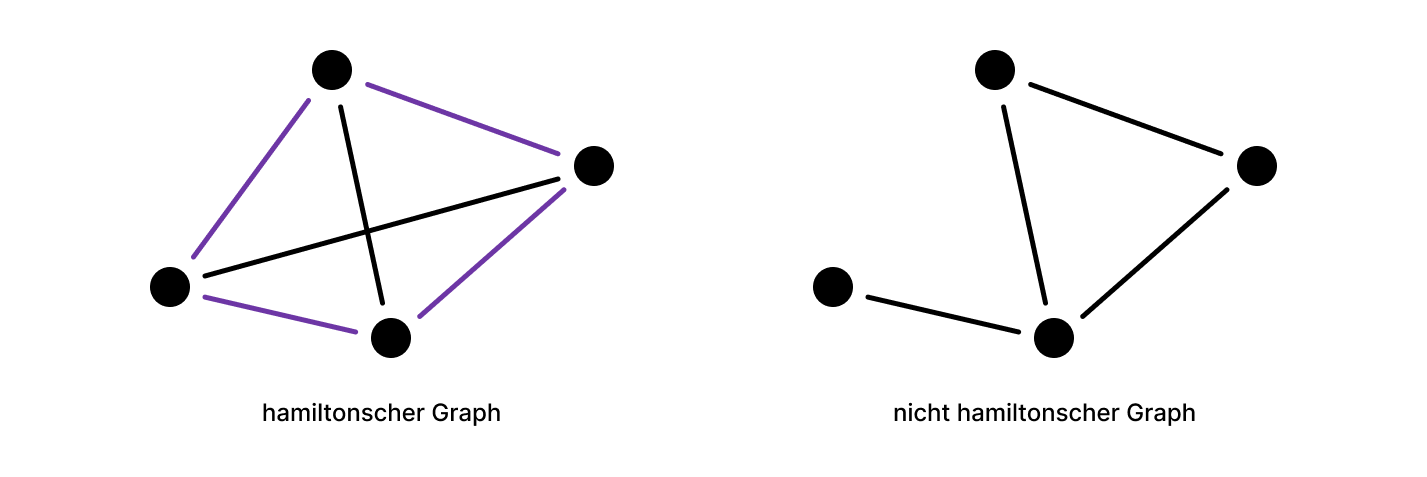
\includegraphics[width=1\textwidth]{content/img/Research/Graphen/HamiltonscherGraph.png}
    \caption{Graph mit Zyklus, welcher alle Knoten beinhaltet (links); kein Hamiltonscher Kreis möglich (rechts)}
    \label{fig:hamiltonsche}
\end{figure}
\FloatBarrier